\documentclass[a4paper,10pt]{article}
\usepackage{graphicx}
\usepackage{geometry}
\usepackage[UTF8]{ctex}
\usepackage{setspace}
\usepackage{titlesec}
\usepackage{enumitem}
\usepackage{hyperref}
\usepackage{fontawesome5}

\geometry{margin=0.8in}
\setstretch{1.5}
\setlist[itemize]{noitemsep, topsep=0pt, leftmargin=*}

\titleformat{\section}{\large\bfseries}{}{0em}{}[\titlerule]
\pagestyle{empty}

\hypersetup{
    colorlinks=true,
    urlcolor=blue,
}

\begin{document}

\noindent
\begin{minipage}[t]{0.72\textwidth}
    \vspace{0pt} % 确保顶部对齐
    {\LARGE \textbf{晏梓铭}} \\[16pt] % 调整姓名与信息间距
    \begin{tabular}{ll}
        \faPhone*~+86 13181337677 & \href{mailto:zimingy3@outlook.com}\faEnvelope*~{zimingy3@outlook.com} \\ 
        \faGithub~\href{https://github.com/yzmyyds}{github.com/yzmyyds} & \faUser~中共预备党员 \\
        \faWeixin~wxid\_jgqzdoo9zwsk22 & \faMapMarker~山东省济宁市 \\
    \end{tabular}
\end{minipage}%
\hfill
\begin{minipage}[t]{0.22\textwidth}
    \vspace{0pt} % 同样保持顶部对齐
    \centering
    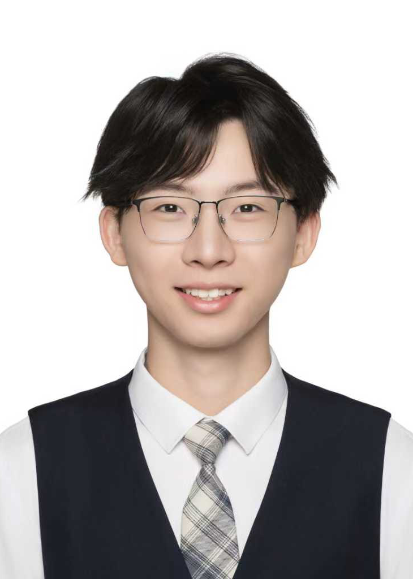
\includegraphics[width=2.4cm,height=3.6cm]{Figures/Photo_2inch.png}
\end{minipage}
\section*{个人简介}
\noindent
具备\textbf{机器人、嵌入式系统、机器学习}等领域实战经验,熟悉控制系统设计与优化。曾主导机械臂抓取控制、无人机结构测试、嵌入式通信架构等项目,精通C/C++、Python、MATLAB,熟悉CAN总线、PCB设计及模型部署,能将算法与硬件高效结合。
\section*{教育背景}
\noindent
\textbf{南洋理工大学(NTU)} \hfill 2025.08 - 至今 \\
电气与电子工程硕士(EEE Global Excellent Award) \\
\textbf{浙江大学(ZJU)} \hfill 2021.09 - 2025.06 \\
电气工程及其自动化学士(GPA 3.9/4.0),\textit{荣誉:} 学习标兵、进步标兵、优秀团支书 \\
\textbf{伊利诺伊大学香槟分校(UIUC)} \hfill 2023.08 - 2023.12 \\
Electrical Engineering (GPA 3.6/4.0),\textit{荣誉:} Dean's List
\section*{技能专长}
\noindent
\textbf{编程语言:} C/C++、Python、MATLAB (Simulink)、SystemVerilog、LC-3汇编、PyTorch \\
\textbf{工具与系统:} Linux、GitHub、Fusion 360、KiCad、JLCEDA、LaTeX \\
\textbf{硬件与嵌入式:} STM32开发、CAN总线、PCB设计、电机控制

\section*{项目经历}
\noindent
\textbf{浙江理工大学先进技术研究院(Internship)} \hfill 2025.02 -- 2025.06 \\
设计并实现双足机器人CAN通信架构,提升信号稳定性。负责四旋翼无人机结构稳定性测试,提出并验证减少振动的结构优化方案。

\noindent
\textbf{毕业设计:基于VR与机械臂的人机交互抓取系统} \hfill 2024.09 -- 2025.06 \\
基于压力传感器反馈开发机械爪抓取/释放控制软件,实现实时稳定抓取。集成VR输入、控制器与步进电机的CAN通信;项目代码与演示视频已开源。

\noindent
\textbf{本科论文:基于机器学习的航空发动机推力预测} \hfill 2024.09 -- 2025.06 \\
搭建并比较随机森林、SVR、XGBoost、决策树、MLP、LSTM模型,调优并集成使预测精度提升约15\%。

\noindent
\textbf{FPGA游戏开发 (ECE 385 Final Project)} \hfill 2024.02 -- 2024.06 \\
使用SystemVerilog设计并实现游戏逻辑,在Intel DE2-115 FPGA开发板上部署,实现横屏格斗游戏。

\noindent
\textbf{学生科研训练计划(SRTP)} \hfill 2023.09 -- 2023.12 \\
搭建基于CNN的图像识别模型,实现无标签图像内容自动摘要。进行深度学习文献调研与Python原型开发。

\end{document}